% Chapter 5 Experimental Setup

\chapter{EXPERIMENTAL SETUP} \label{ch5}

In this chapter, we discuss the method used to measure the complexity
of any given race track following which we move on to describe tracks
developed for performing our experiments using the custom environment
discussed in Chapter \ref{ch4}. We have developed 5 different types of
tracks in two levels of complexity. The first level of complexity is
called `Basic Tracks' . The second level of tracks are inspired by AWS
Deepracer \cite{deepracer} challenge tracks and are inspired by real
world race tracks with much higher level of complexity and are
labelled `Complex Tracks'.


\section{TRACK COMPLEXITY MEASURE}

Before proceeding with the Basic and Complex Tracks, we will introduce
the features used to quantify the complexity of a track. Features
indicating the complexity of the track in decreasing order of
complexity are as follows:
\begin{enumerate}
\item Chicanes
\item Sharp Turns
\item Sweeping Turns
\item Distance of Track
\end{enumerate}

\subsection{Chicanes}
Chicanes refer to a tight sequence of corners in alternate
directions. They are usually inserted into a circuit to slow the cars,
often just before a high-speed corner \cite{F1Chicane}. These are the
most complex for the agent to navigate due to slow speed required and
precise control of the turn inputs in order to pass the chicane
without hitting the sidewalls of the track. The leeway for error is
the least when navigating a chicane due to this nature. Figure
\ref{fig:chicane} depicts an example of a chicane.
\begin{figure}[H]
  \centering 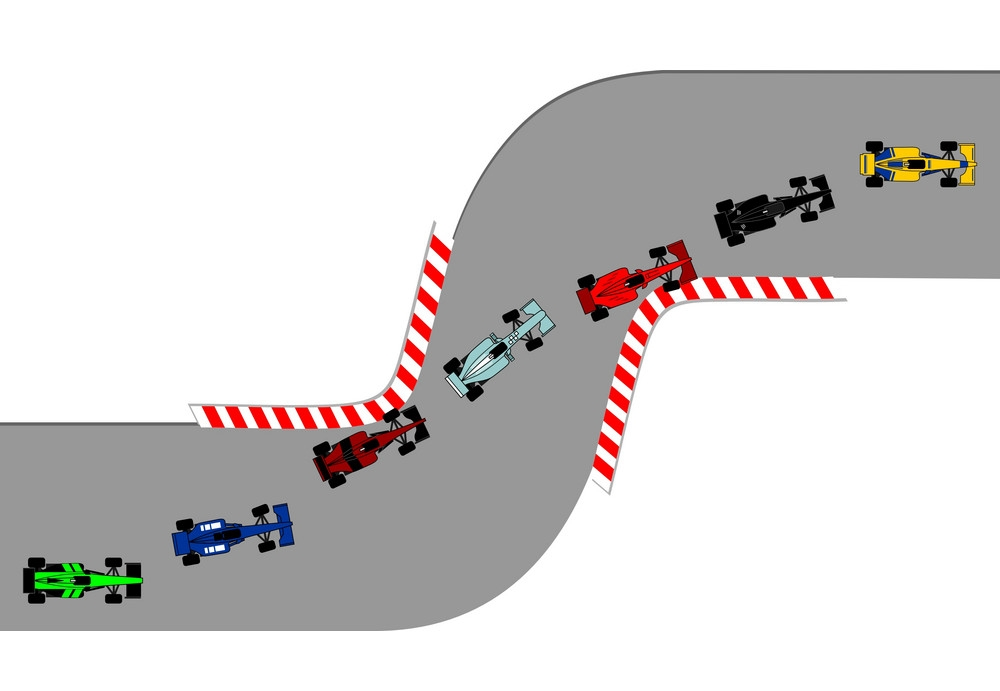
\includegraphics[width=0.7\textwidth]{images/Chicane.jpg}
  \caption{Chicane example (Image from
    \href{https://www.vectorstock.com/royalty-free-vector/chicane-road-circuit-vector-7128004}{Vector
      Stock})}
  \label{fig:chicane}
\end{figure}

\subsection{Sharp Turns \& Sweeping Turns}
The difference betwen Sharp Turns and Sweeping Turns is the radius of
the turn. Turns with a lower radius are more difficult to navigate and
the average speed of the car (agent) is lower and these are called
sharp turns. Sweeping turns are turns having a larger radius of
curvature allowing for faster speeds and minimal steering input
allowing for more leeway for errors in the inputs. Figure
\ref{fig:turns} shows the different types of turns.

\begin{figure}[H]
  \centering
  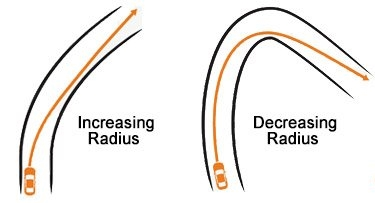
\includegraphics[width=0.5\textwidth]{images/Turn-Types-crop.jpg}
  \caption{Sweeping vs Sharp Turns (Image from
    \href{https://go-kart-source.com/go-kart-cornering/}{Go-Kart-Source})}
  \label{fig:turns}
\end{figure}

\subsection{Distance}
Distance of the track is the least important feature for track
complexity. For the same given distance, the presence of more chicanes
and/or turns determines the real world complexity in navigating the
track. Thus, distance of the track is the least important feature to
determine the complexity of a track. However, it is to be noted that
longer the distance, the chances for making a mistake increases due to
the time taken to complete a lap around the track.

\subsection{Computing Complexity}
In order to quantify the complexity of a track, we use a custom metric
given by
\begin{equation}
    Complexity = (4 \times Chicanes) + (2 \times SharpTurns) + SweepingTurns     
\end{equation}

% +  \frac{10 \times TotalTurns}{distance}
The complexity of all the tracks developed in our custom environment
are provided in Table~\ref{tab:complexity}.

\section{BASIC TRACKS} \label{ch5-basictrack}
%
In this section, we cover the basic tracks we developed as a part of
Phase I of our experimentation. We developed the Oval track, shown in
Figure~\ref{fig:ovaltrack}, which is the simplest of the tracks in
terms of layout as a proof of concept tracks to ensure all our
supporting systems like the checkpointing systems were working as
expected in our custom built environment. To test the the agent
behaviour when more complicated maneuvers are required, we developed
the One-Kink Track and Two-Kink track as shown in
Figures~\ref{fig:onekink} and \ref{fig:twokink}.

\begin{figure}[H]
  \centering
  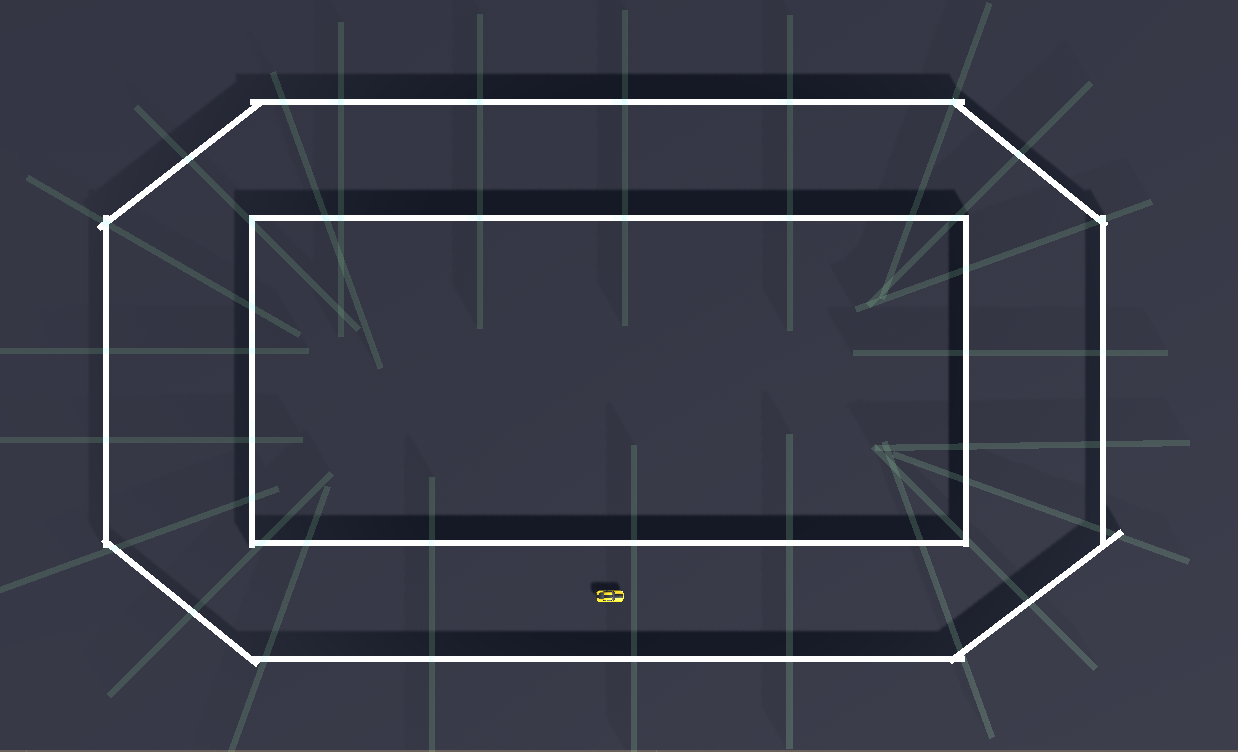
\includegraphics[width=0.90\textwidth]{images/tracks/OvalTrack.png}
  \caption{ Oval Track}
  \label{fig:ovaltrack}
\end{figure}
\begin{figure}[H]
  \centering
  \begin{minipage}[b]{0.45\textwidth}
    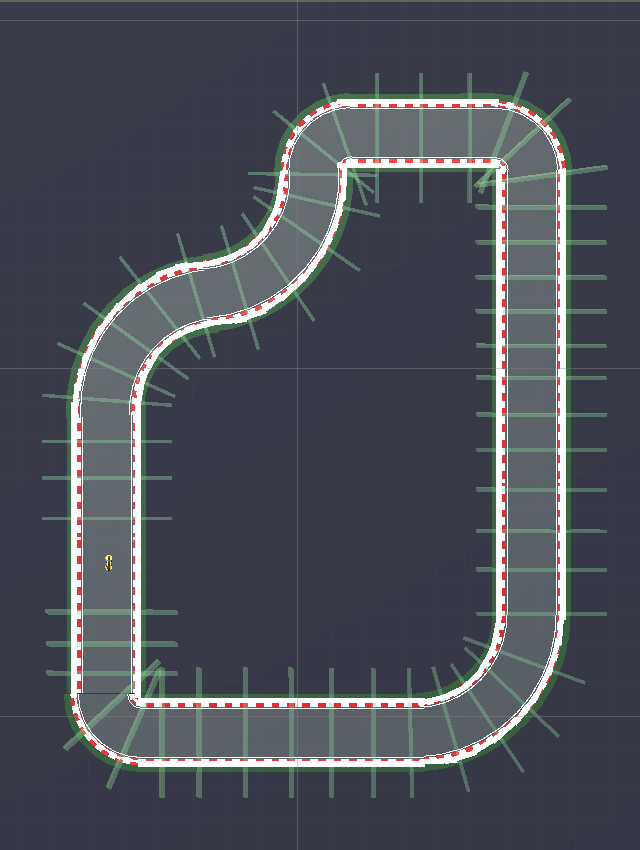
\includegraphics[width=\textwidth]{images/tracks/ComplicatedTrack.PNG}
    \caption{One Kink Track}
    \label{fig:onekink}
  \end{minipage}
  \hfill
  \begin{minipage}[b]{0.45\textwidth}
    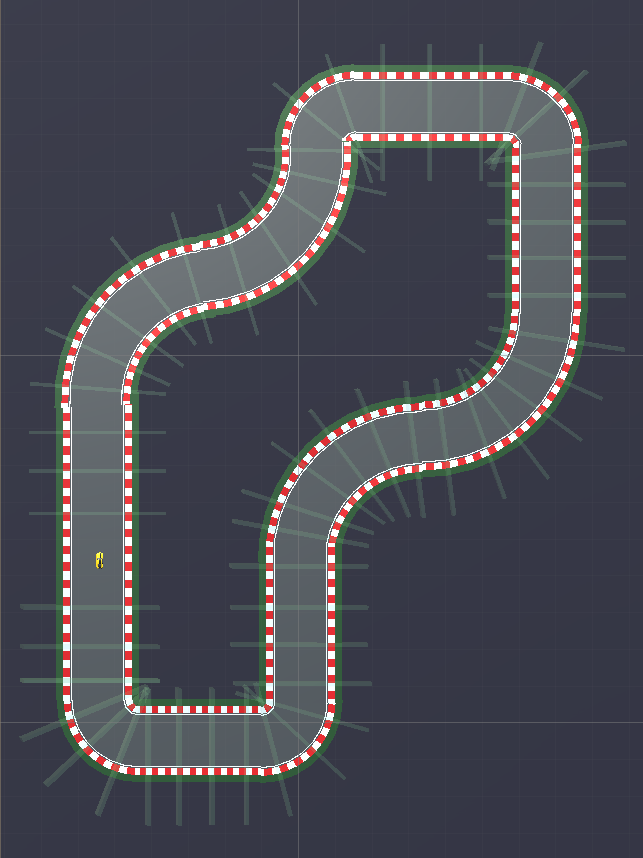
\includegraphics[width=\textwidth]{images/tracks/EvenMoreComplicatedTrack.PNG}
    \caption{Two Kink Track}
    \label{fig:twokink}
  \end{minipage}
\end{figure}

\section{COMPLEX TRACKS}
%
For developing `complex tracks', we have used a real world Formula 1
race track of Barcelona and a track used as a part of AWS deepracer
challenge namely AWS Asia Pacific Track to serve as inspirations to
test the agent performance in tracks closer to real world. These
tracks are longer and feature more complicated track layout in
comparison to the basic tracks discussed in section
\ref{ch5-basictrack}.
\begin{figure}[H]
  \centering
  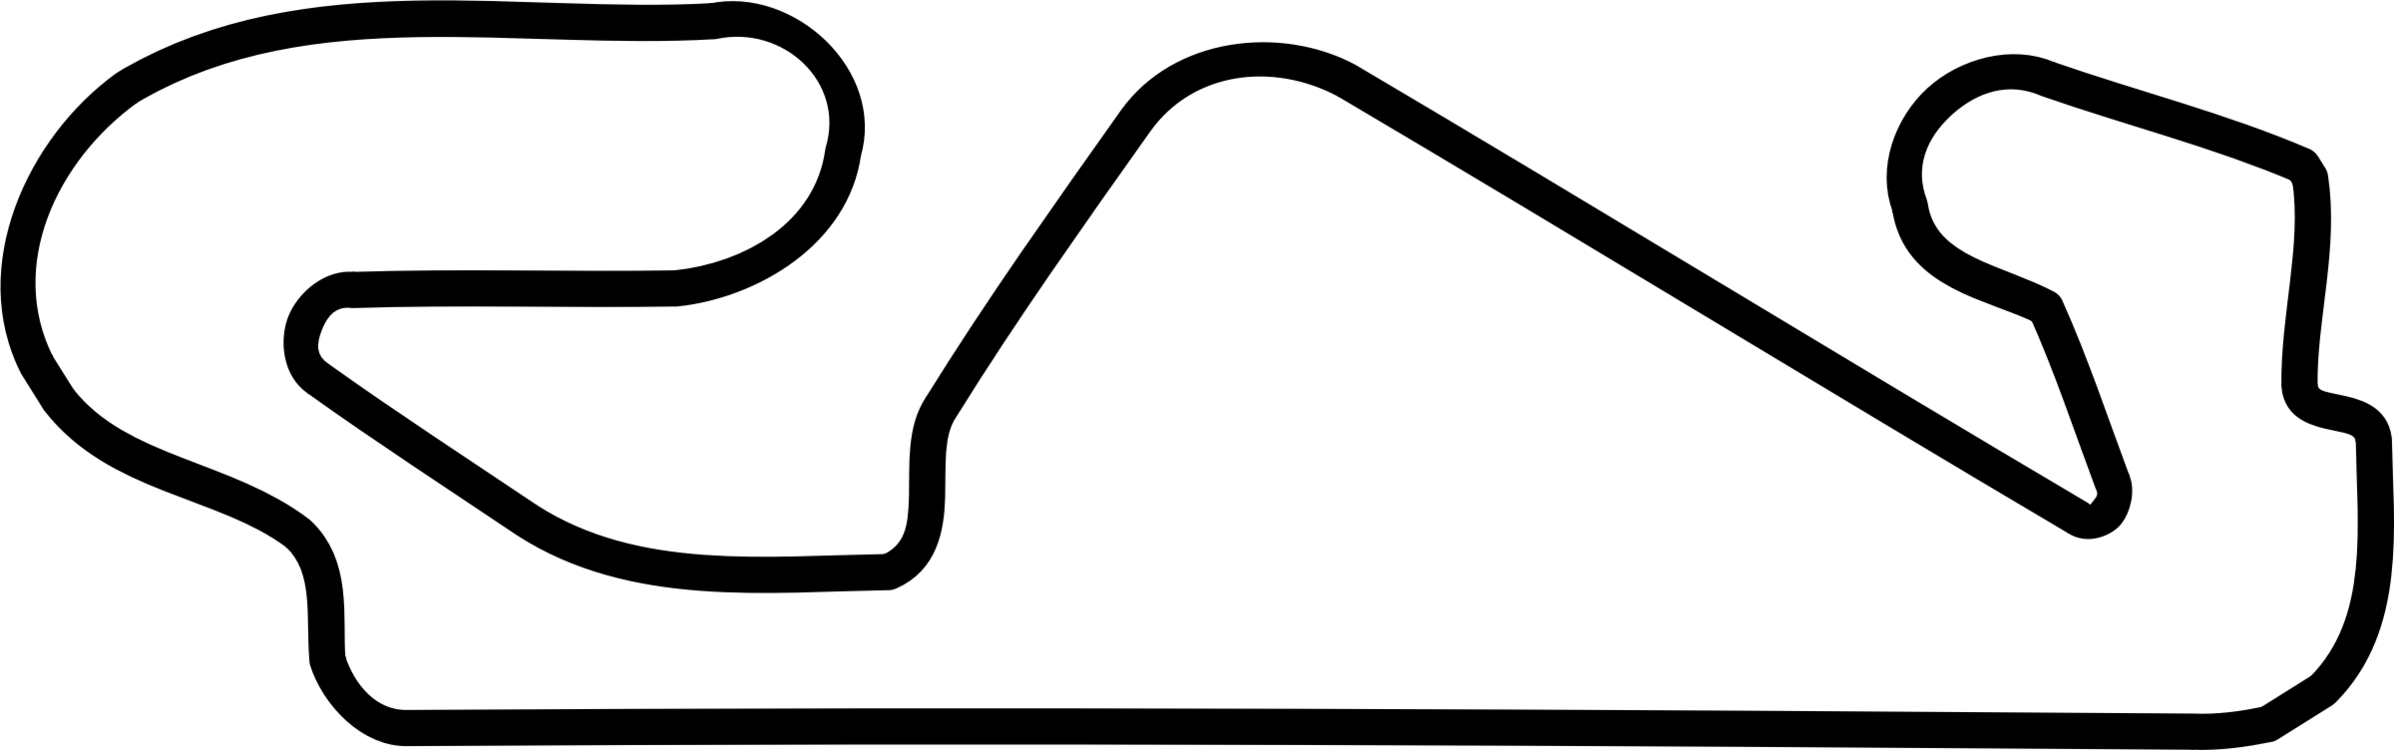
\includegraphics[width=1.0\textwidth]{images/tracks/BarcelonaOG.png}
  \caption{Original Barcelona Racetrack (Image from
    \href{https://www.clipartmax.com/download/m2H7G6d3Z5A0G6d3_circuit-de-barcelona-catalunya-el-circuit-restaurant-barcelona-f1-circuit-map/}{Clipartmax})}
  \label{fig:barcelona}
\end{figure}

\begin{figure}[H]
    \centering
    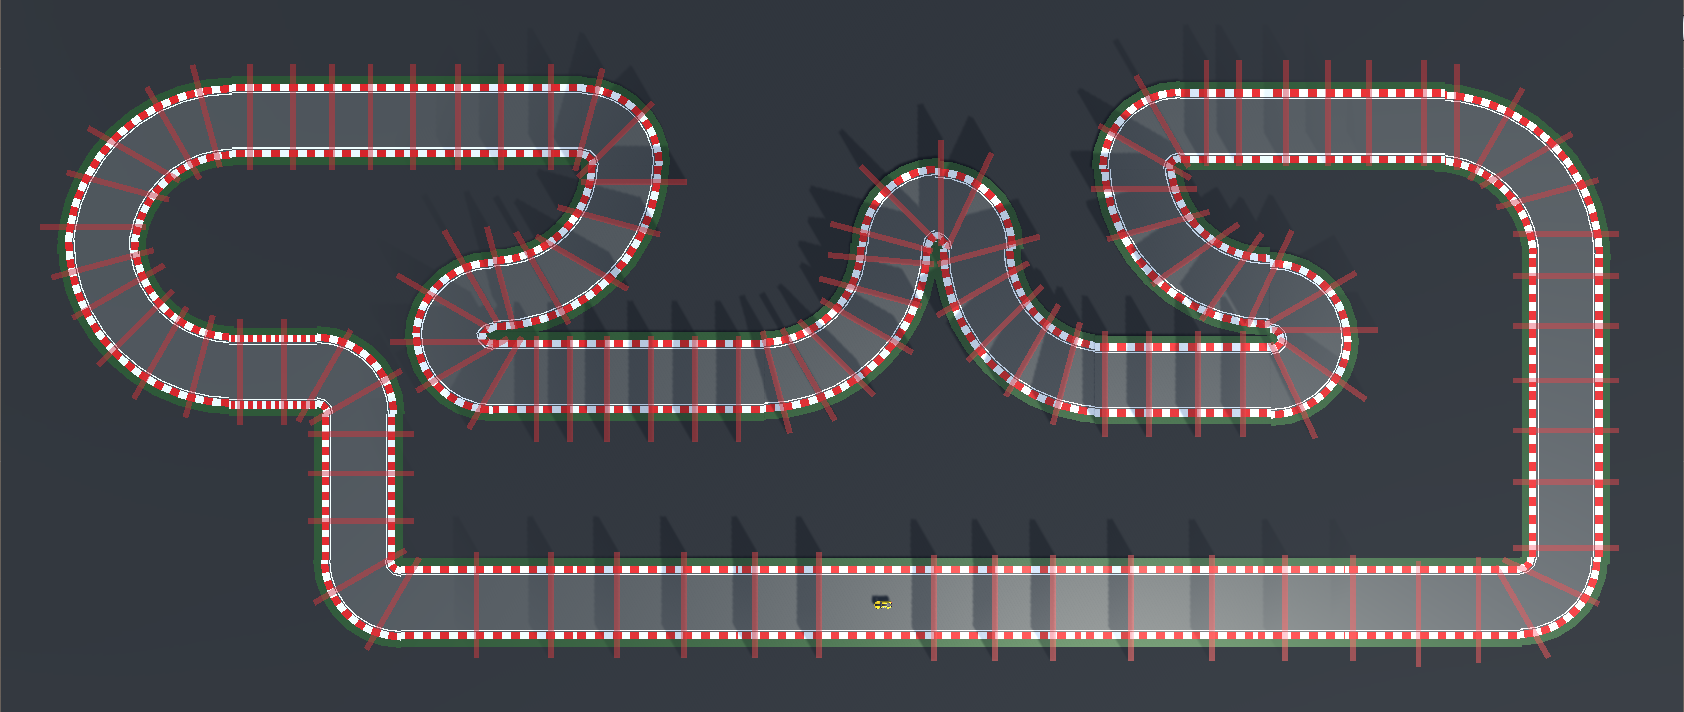
\includegraphics[width=1.0\textwidth]{images/tracks/Barcelona.png}
    \caption{Barcelona Track in Unity}
    \label{fig:barcelona}
\end{figure}

\begin{figure}[H]
    \centering
    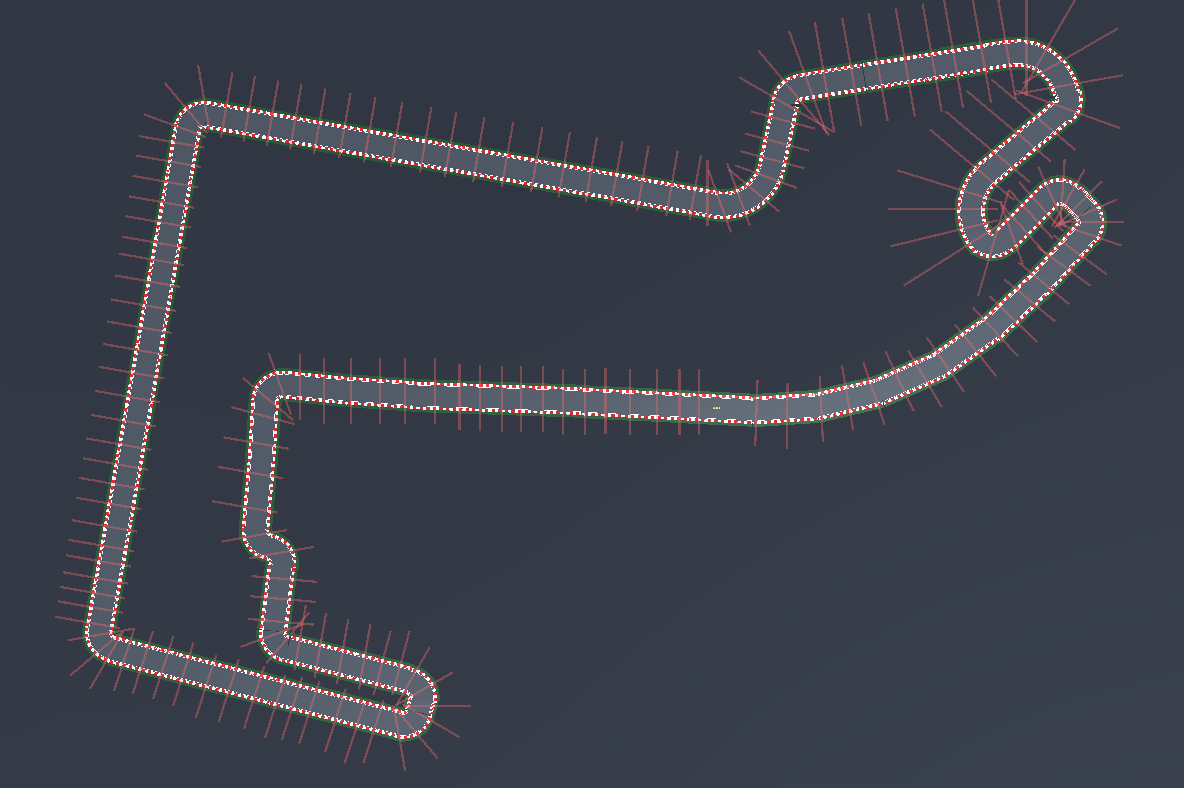
\includegraphics[width=0.9\textwidth]{images/tracks/AWSTrack.png}
    \caption{AWS Asia Pacific Track}
    \label{fig:awstrack}
\end{figure}


\begin{table}[H]
\centering
\begin{tabular}{|p{1.9cm}|p{2.5cm}|p{2cm}|p{1.8cm}|p{2cm}|p{3.5cm}|}
\hline
\textbf{Type}                                         & \textbf{Track} & \textbf{Chicanes (C)} & \textbf{Sharp Turns (SH)} & \textbf{Sweeping Turns (SW)} & \textbf{Complexity \newline (4C+2SH+SW)} \\ \hline
\multicolumn{1}{|c|}{\multirow{3}{*}{\textbf{Basic}}} & Oval     & 0                     & 4                         & 0                            & 8                                      \\ \cline{2-6} 
\multicolumn{1}{|c|}{}                                & One Kink       & 1                     & 3                         & 1                            & 11                                     \\ \cline{2-6} 
\multicolumn{1}{|c|}{}                                & Two Kink       & 2                     & 4                         & 0                            & 16                                     \\ \hline
\multirow{2}{*}{\textbf{Complex}}                     & Barcelona      & 0                     & 8                         & 6                            & 22                                     \\ \cline{2-6} 
                                                      & AWS Track      & 1                     & 8                         & 4                            & 24                                     \\ \hline
\end{tabular}
\caption{Complexity of the various tracks developed}
\label{tab:complexity}
\end{table}

% \section{AGENT INPUTS}

% The agent in our environment is the Car(1) itself. The car makes decisions such as when to accelerate and when to brake based on the inputs that it receives. The two inputs that the agent receives are the current speed and the Ray Perception inputs(4) from the sensors placed on the car. The Ray Perception inputs inform the car of the distance of the object, and also what kind of object it is. For example, the object could be a Checkpoint(2) or a SideWall(3). The car can make use of this information to decide when to accelerate, brake, or turn.


\section{ML AGENTS}
MLagents is an open source package that provides a framework to train
and develop intelligent agents in the Unity game engine
environment. It supports multiple methods of training intelligent
agents using reinforcement learning, imitation learning, and other
machine learning methods through the Python API provided. ML Agent
contains 4 major components as shown in Figure~\ref{fig:mlagents}.
%
\begin{figure}[H]
  \centering
  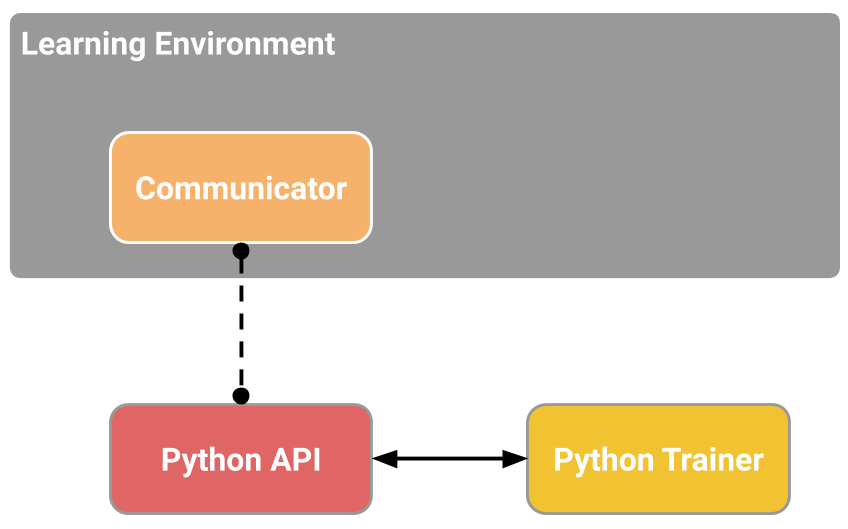
\includegraphics[width=1.0\textwidth]{images/mlagents.png}
  \caption{Components of ML Agents Framework (Image from
    \href{https://github.com/Unity-Technologies/ml-agents}{ML Agents
      Github})}
  \label{fig:mlagents}
\end{figure}

\begin{itemize}
\item \textbf{Learning Environment} refers to the Unity scene created
  for experimentation. This scene serves as the environment for the
  agent to interact with and receive observations and take actions in.
\item \textbf{External Communicator} feeds the data from the Unity
  scene and passes it on to the Python API
\item \textbf{Python API} provides for a method to directly access
  the Learning Environment from the external Python code to interact
  and manipulate the learning environment
\item \textbf{Python Trainer} is the place where the Algorithm used
  to train the agent is located. The algorithm has access only to the
  Python API and are written using PyTorch \cite{Pytorch}
\end{itemize}

\section{PPO NETWORK AND HYPER-PARAMETERS}

The algorithm we use to train our agents in the environment is the PPO
Algorithm covered in Section~\ref{ch4-ppo-alg}. PPO Contains two
function approximators representing the actor and the critic
respectively and these are developed using the neural networks as
shown in Figure~\ref{fig:ppo-network}. Both the networks consist of 3
layers with 256 hidden units present in each of the layers. The Actor
network returns the action probabilities and the Critic returns the
value function.

\begin{figure}[H]
    \centering
    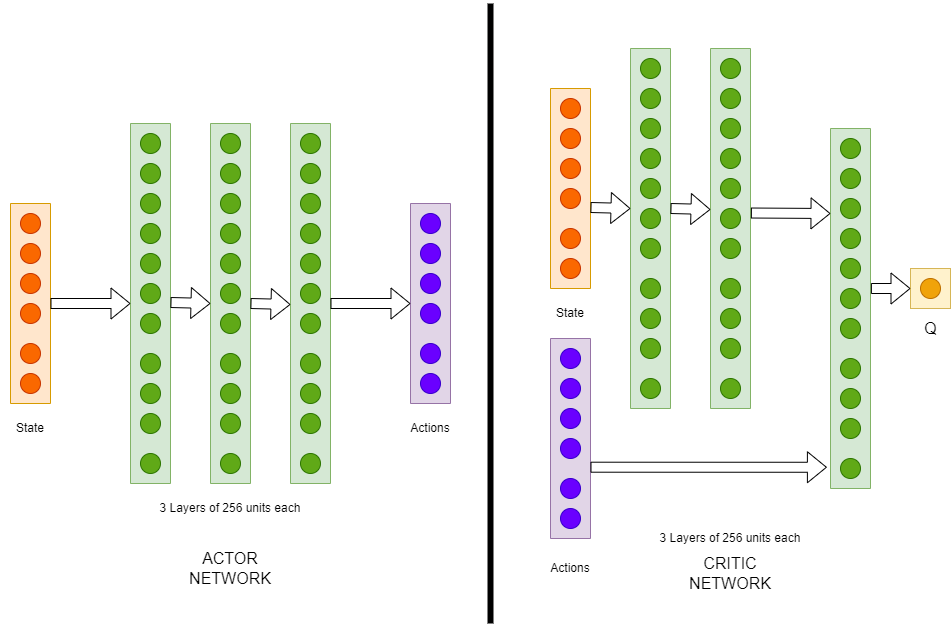
\includegraphics[width=1.0\textwidth]{images/ppo-network-v2.png}
    \caption{PPO Network Architecture}
    \label{fig:ppo-network}
\end{figure}

All the models were trained for 8-12 million steps depending on
complexity. A batch size of 1024 was used with a buffer which stores
experiences before making updates of the size 10240. All the agents
were trained using 3 passes of the experience buffer to improve the
stability of the training. Training episode ends when the reward
accumulated becomes negative ($R < 0$) or if the agent successfully
completed a lap around track. At episode completion, the progress of
the agent is reset on the track and the agent is reset at start
location with 0 initial velocity. We use an initial learning rate of
$3 \times 10^{-2}$ with a linear learning rate scheduler to ensure
that the updates are not to large with the progress.

